% Created 2021-12-21 Tue 11:31
% Intended LaTeX compiler: pdflatex
\documentclass[11pt]{article}
\usepackage[utf8]{inputenc}
\usepackage[T1]{fontenc}
\usepackage{graphicx}
\usepackage{longtable}
\usepackage{wrapfig}
\usepackage{rotating}
\usepackage[normalem]{ulem}
\usepackage{amsmath}
\usepackage{amssymb}
\usepackage{capt-of}
\usepackage{hyperref}
\author{Prashant Tak}
\date{\today}
\title{Notes - URLLC Optimization}
\hypersetup{
 pdfauthor={Prashant Tak},
 pdftitle={Notes - URLLC Optimization},
 pdfkeywords={},
 pdfsubject={},
 pdfcreator={Emacs 27.2 (Org mode 9.6)}, 
 pdflang={English}}
\begin{document}

\maketitle
\setcounter{tocdepth}{2}
\tableofcontents \clearpage
\section{Methodology}
\label{sec:org036007b}
\begin{itemize}
\item Read first two sections and conclusion
\item Most Papers talk about Channel Access Delay but we want to minimze network delay
\end{itemize}
\section{TODO}
\label{sec:org1ec20c0}
\subsection{Lookups - Paper Wise}
\label{sec:orgf6bb34b}
\subsubsection{1}
\label{sec:org1a11f6f}
\begin{itemize}
\item Physical Layer Channel Modeling
\item URLLC Trans Schemes
\item PDP (Power Delay Profile), Delay Spread
\end{itemize}
\subsection{Lookup}
\label{sec:org20d26f6}
\begin{enumerate}
\item Schemes
\item OFDMA Systems
\item SINR
\item Define system Params in Network Dummies
\end{enumerate}
\subsection{Reading}
\label{sec:orgd24ecc7}
\begin{itemize}
\item Ch-6 CompNet Notes (Aloha - 6.4.3)
\end{itemize}
\section{Spreadsheet}
\label{sec:org8b0b589}
\begin{center}
\begin{tabular}{rllll}
S. No. & Title & Target Problem & Approach Used & Limitations\\
\hline
1 & UR Comm for Ind IoT &  &  & \\
2 & Res Alloc \& HARQ Opt for URLLC Traffic &  &  & \\
3 & Delay Aware Pr Access Class for mMTC &  &  & \\
4 & QoS \& Privacy Aware Routing for Ind IoT &  &  & \\
5 & QoS Diff Scheduling of URLLC under FIFO &  &  & \\
6 & Priority S-ALOHA for URLLC &  &  & \\
7 & Min Delay Violation in URLLC for fading chann &  &  & \\
8 & URLLC and eMBB coexist in unlicense spectrum &  &  & \\
9 & Delay Perf of MISO Wireless comm &  &  & \\
10 & Enabling Critical mMTC &  &  & \\
\end{tabular}
\end{center}
\section{Shared by Ma'am}
\label{sec:org2dbd1dc}
\subsection{Ultra Reliable Comm for Industrial IoT}
\label{sec:org0328597}
\subsubsection{Readings}
\label{sec:orgab35c35}
\begin{enumerate}
\item \url{https://en.wikipedia.org/wiki/Diversity\_scheme}
\item 
\end{enumerate}
\subsubsection{Abstract}
\label{sec:org7b62d7f}
\begin{itemize}
\item Factory Automation, Smart Factories, Automated Warehouses
\item Diversity for high reliability, short packets for low latency,  On-the-fly Channel Estimation, Decoding for fast receiver processing.
\item Ray Tracing Channel Simulation
\end{itemize}
\subsubsection{Introduction}
\label{sec:org3947f49}
\begin{enumerate}
\item Their Lit Review
\label{sec:orgbf0498f}
\begin{itemize}
\item Factory automation merges operational, information, and communication technologies with cyber-physical systems.
\item Main Diff: Focus on mMTC and URLLC for machine connectivity.
\item URLLC vital for mission-critical communications (Latency of 1ms with 99.999\% reliability)
\item URLLC Transmission Schemes:
\begin{enumerate}
\item Diversity Techniques
\item Short Packets within a short TTI (Trans Time Intvl)
\item Fast Receiver Processing (Turbo codes for data channel and polar codes for control channels)\footnote{The common control channel (CCCH), used for transmission of control information in conjunction with random access. The dedicated control channel (DCCH), used for transmission of control information to/from a device. \href{https://klevas.mif.vu.lt/\~skersys/vsd/turbo/0429hage.pdf}{Paper about Coding}}
\end{enumerate}
\item Physical Layer Channel Modeling for design and evaluation of URC.
\item This work emphasizes that the abundance of metallic scatterers present in the industrial environment causes dense multipath scattering.
\item Special Topology and Dense Metallic Scatterers are significant differences between ind, office and residential propogation environments.
\item Temporal evolution of Rich Multipath Components (MPCs) in delay domain, neglecting space domain.
\end{itemize}
\item Proposal
\label{sec:org626e985}
\begin{itemize}
\item 5G system arch for IIoT services in automated warehouse.
\item Use Cases: Sensor Monitoring, Cooperative Motion Control, Video Operated Remote Control
\item Transmission Scheme Evaluation by RT channel models at 28 and 60 GHz.
\item Time evolution of delay and doppler power spectra over automation process presented
\end{itemize}
\item Organization
\label{sec:org15fc1ef}
\begin{itemize}
\item Proposed Model
\item Use Cases Presented
\item Channel Model Requirements
\item Analysis
\end{itemize}
\end{enumerate}
\subsubsection{5G CommSys For IIoT}
\label{sec:org5760987}
\begin{enumerate}
\item System Architecture
\label{sec:orgbb14157}
\begin{itemize}
\item Components of system
\begin{enumerate}
\item Access: Provides radio connectivity between devices and 5G access nodes.
\item Transport Network: Interconnected via backbone nodes which carry information from access nodes to hosting cloud
\item Management
\item Cloud: Poweful processing capabilities that allow for storage, management.
\item Applications: Data Storage and sharing, order entry, inventory management, financial accounting features. (Robot Grippers - Usecase: Quicker, reliable motion)
\end{enumerate}
\end{itemize}
\begin{center}
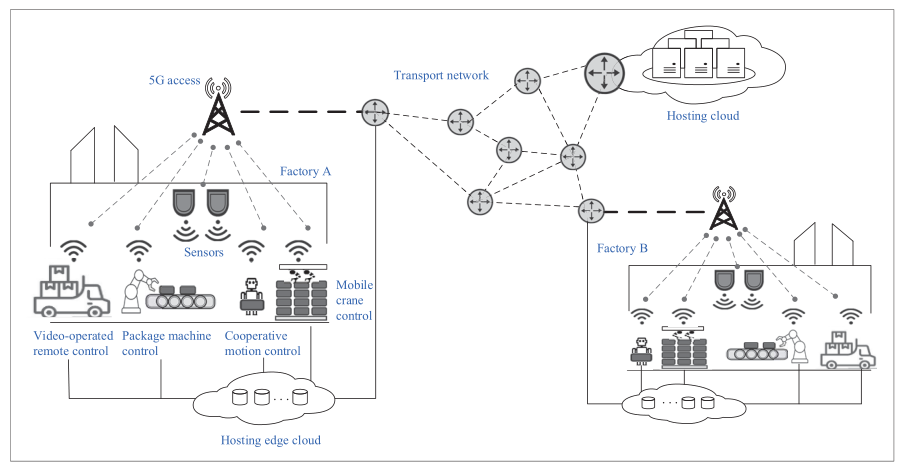
\includegraphics[scale=0.50]{./assets/p1f1.png}
\end{center}
\begin{itemize}
\item Considered Use Cases (Differing Latency Bounds)
\begin{enumerate}
\item Package Machine Control
\item Cooperative Machine Control
\item Mobile Crane Control
\item Video-Operated RC
\end{enumerate}
\end{itemize}
\item Key Technologies for URLLC-Based Services
\label{sec:org89a5c90}
\begin{itemize}
\item Requirements: In \texttt{L} seconds, data packets having atmost \texttt{B} bytes transferred with a delay < \texttt{D} seconds in 99.9999\% attempts.
\item Diversity/Redundancy:
\end{itemize}
\item Industrial Channel Model
\label{sec:org4f69017}
\begin{enumerate}
\item Requirements
\label{sec:org7224104}
\begin{enumerate}
\item Extreme Frequency Range
\item Ultra-wide Bandwidth
\item Support of massive MIMO antenna array
\item Spatial Consistency
\end{enumerate}
\item Modeling and Characteristic analysis
\label{sec:org633c543}
\begin{itemize}
\item For use-cases, Video-operated RC and Coop Motion Control
\item The mobile robots travel in different alleys to find the required objects.
\item When they are moving, the video-operated RC supports the autonomous navigation to detect any collisions and stop it immediately.
\item After mobile robots come to layered shelves with the needed item, they're under cooperative motion control to detect items, pick them up, or drop them.
\end{itemize}
\item FIXME RT Simulation
\label{sec:org16d9523}
\begin{itemize}
\item Inherently spatially consistent
\item Only few material parameters to be calibrated by measurements
\item HPC CloudRT: \url{http://raytracer.cloud/}
\end{itemize}
\begin{center}
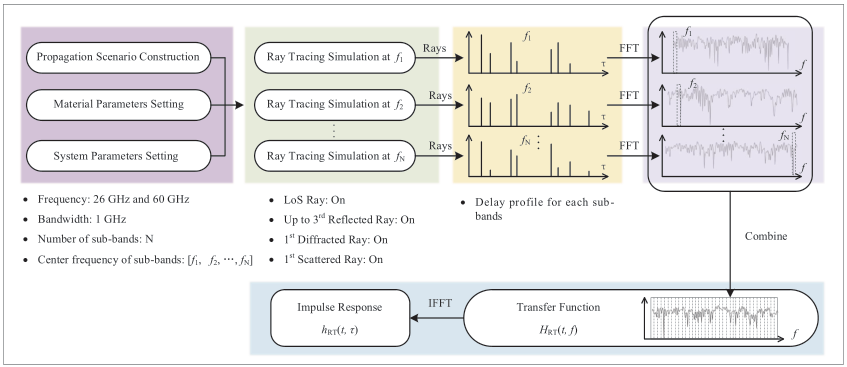
\includegraphics[width=.9\linewidth]{./assets/p1f2.png}
\end{center}
\begin{itemize}
\item 
\end{itemize}
\end{enumerate}
\end{enumerate}
\subsubsection{Conclusion}
\label{sec:org6b9fa38}
Due to shorter wavelength of 60 GHz, reflected MPCs with high power increase, and then the strong paths supporting reliable radio links are enhanced. Diversity in frequency and space dimensions are demonstrated where 60 GHz channel has high diversity orders, and has possible effective combining at end user level.
\subsection{Resource Allocation and HARQ Optimization for URLLC Traffic in 5G Wireless Network}
\label{sec:org97ff87c}
\subsubsection{Abstract}
\label{sec:org6d65d3d}
\begin{itemize}
\item URLLC Requirements:
\begin{enumerate}
\item Low Packet Delays (< 1ms)
\item High Reliability (\textasciitilde{}99.999\%)
\end{enumerate}
\item \emph{Downlink}\footnote{Link from satellite to ground station or transmission path from cell site to cell phone.} URLLC traffic using queuing network-based model for wireless system.
\item Effect of design choices on:
\begin{enumerate}
\item System Parameters (Bandwidth, Link, SINR(Signal to interference plus noise ratio), QoS)
\item Resource Allocation Scheme in OFDMA (Orthogonal FQ Division Multiple Access) systems
\item Hybrid Automatic Repeat Request Schemes (HARQ is combination of high-rate Fwd Error Correction and Automatic Repeat Request Error-Control)
\end{enumerate}
\item Focus on:
\begin{enumerate}
\item Minimum bandwidth to support given URLLC load scale with associated QoS constraints
\item Characterization of optimal OFDMA resource allocation schemes that maximize admissible URLLC load
\item Optimization of a repetition code-based packet re-transmission scheme.
\end{enumerate}
\end{itemize}
\subsubsection{Introduction}
\label{sec:org43ef5cf}
\begin{itemize}
\item URLLC Applications: Industrial Automation, Mission Critical Traffic, VR, etc.
\item Downlink transmission of URLLC traffic in FDD (Freq Division Duplex) with separate fq bands for uplink and downlink is considered.
\item QoS Requirements: Packet Size \texttt{L} bits, Max. end-to-end delay between Rx and BS: \texttt{d} secs, Probability= 1-\(\delta\).
\item Typical Values: L=32 bytes, d=1ms, \(\delta\) = 10\textsuperscript{-6}.
\item Delay includes: Queuing delay at BS, transmission duration, rx processing delay, packet decoding feedback transmission duration, time to make further transmissions.
\item Studies the impact of design choices on URLLC \emph{capacity} (load). Impact of:
\begin{enumerate}
\item Sys BW: \texttt{W}, User SINR, QoS Params \texttt{d}, \(\delta\).
\item \emph{Resource allocation} in time-fq plane of OFDMA (packets are allocated different parts of a time-fq plane for data transmission) system.
\item HARQ schemes on URLLC Capacity.
\end{enumerate}
\item A URLLC packet can be scheduled as \emph{tall} transmissions which use large W over longer d or \emph{wide} trnsms that use small W for short d.
\item Tall trnsms result in reduced tx times for packets but number of concurrent trx also reduces which might result in queuing or blocking of URLLC packets due to unavailability of W.
\item Wide trxs permit higher number of concurrent trxs but with longer trxs times for each packet which may lead to bandwidth scarcity.
\item HARQ schemes' analysis might help in evaluating max. no. of re-trxs allowed and reliability (coding scheme) to be targeted after each trx.
\end{itemize}
\subsection{Delay-aware Priority Access Classification for Massive Machine-type Communication}
\label{sec:org037df5d}
\section{Initial Picks}
\label{sec:org8b2bb13}
\section{Basics}
\label{sec:org50ebe08}
\subsection{5-G Network (NR: New Radio) (Ref: Intelli Resource Slicing: Deep RL approach)}
\label{sec:orgc5d7bae}
\begin{itemize}
\item Services provided:
\begin{enumerate}
\item \textbf{URLLC} (Ultra-Reliable Low Latency Communication): Target \emph{mission critical} communications such as autonomous vehicles, tactile internet and remote surgery. \emph{Sporadic with short packet size} and \emph{relatively low data rate}. Due to need of LL, they are localized in time with \emph{short transmission time intervals} (sTTI). Requirements: High reliability i.e. PER < 10\textsuperscript{-5} and low latency.
\item \textbf{eMBB} (Enhanced Mobile Broadband): Focus on high data rate application (4K, VR). Extension of LTE-Advanced broadband service that allows for higher data rate and coding over large transmission blocks for a long time interval. Hence, objective: \emph{High data rate with moderate reliability and packet error rate (PER) < 10\textsuperscript{-3}.}
\item \textbf{mMTC} (Massive Machine-Type Communications): Aims at serving large number of IoT devices sending data \emph{sporadically} with \emph{low and fixed uplink transmission rate}. Focus on energy efficiency.
\end{enumerate}
\item Comparison with 4G systems
\begin{enumerate}
\item In 4G systems, control signaling takes a large portion of transmission latency (0.3-0.4ms). So designing a short packet transmission system with latency of 0.5ms might cause waste of > 60\% resources for control overheads\footnote{Data that you send across a wireless network is housed in a data envelope called a \emph{packet}. Each transmission includes additional information, called \emph{overhead}, that is required to route the data to the proper location. Network control mechanisms, such as scheduling, routing, and flow control, ensure effective data transport in a communication network, but also require the exchange of network state information, such as channel conditions and queue-length information, which amounts to \emph{control overhead}. \href{http://cnrg.mit.edu/protocol-information}{REF}}.
\item To support URLLC services, changes in physical layer design of 5G NR systems have been made.
\item \emph{Physical Layer Enabler}
\end{enumerate}
\item Resource Slicing Problem: \\
Aims at maximizing eMBB data rate subject to URLLC reliability constraint, while considering variance of eMBB data rate to reduce impact of immediately scheduled URLLC traffic on eMBB reliability. DRL Approach:
\begin{enumerate}
\item \emph{eMBB resource allocation phase}: Optimization problem decomposed into three subproblems which are each transformed into convex form to obtain \emph{approximate} allocation solution.
\item \emph{URLLC scheduling phase}: DRL based algorithm is proposed to intelligently distribute incoming URLLC traffic among eMBB users.
\end{enumerate}
\item Proposed approach satisfies stringent URLLC reliability while keeping eMBB reliability > 90\%.
\end{itemize}
\subsection{Network Theory for Dummies}
\label{sec:org8b9a01b}
\subsection{Telecommunications}
\label{sec:orga9420a5}
\begin{enumerate}
\item FDM: Technique by which total bandwidth available in communication medium is divided into a series of non-overlapping frequency bands, each of which is used to carry a separate signal. (Allows for quicker transmission and parallelization). \emph{e.g. Radio, Cable TV}.
\item OFDM: Specialized FDM with the additional constraint that all subcarrier signals within a communication channel are orthogonal to each other i.e. \emph{crosstalk} between the sub-channels is eliminated and the inter-carrier guard bands are not needed which simplifies the design of transmitter and receiver. Here a separate filter for each sub-channel is not needed.
\item OFDMA: Multi-user version of OFDM, multiple access is achieved by assigning subsets of subcarriers to individual users which allows for simultaneous low-data rate transmission from several users.
\end{enumerate}
\end{document}
